% !TEX root =  master.tex
\chapter{Analyse der Infrastrukturlösung von SAP Subscription Billing}
\label{Kapitel_Infrastruktur_CF}
Die folgenden beiden Unterkapitel beinhalten den Überblick des technischen Aufbaus der SAP Subscription Billing \ac{SaaS}-Lösung auf der \ac{CF} und die Erläuterung der für die prototypische Portierung relevanten Komponenten. Zudem erfolgt die Evaluation der \ac{CF}-Plattform mittels der in Kapitel \ref{kapitel_merkmale_vorgehensweise} definierten Merkmale und Untersuchungsvorgehensweise.
\section{Technischer Aufbau}
\label{technischer_aufbau_cf}
Die Übersicht des technischen Aufbaus der Infrastrukturlösung ist aus der Grafik \ref{grafik_technischer_aufbau_cf} zu entnehmen.
\begin{figure}[h]
	\begin{center}
		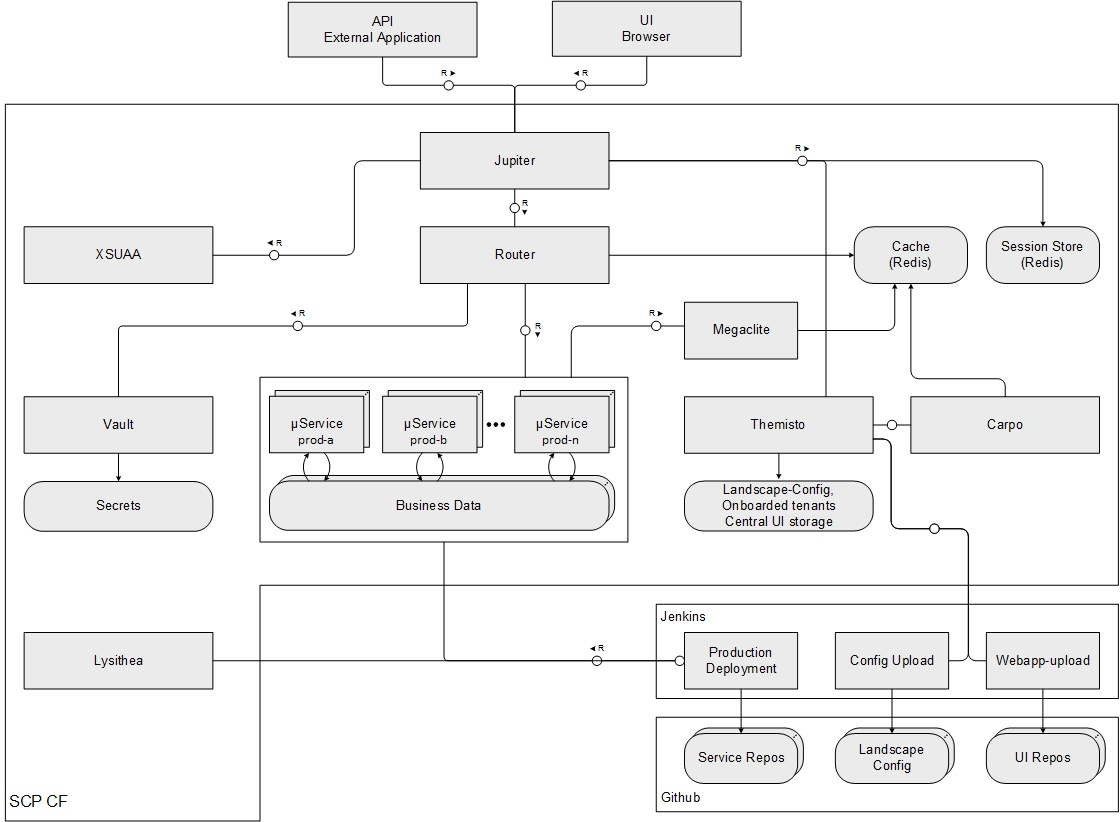
\includegraphics[width=16cm]{img/cf_infrastruktur.JPG}
		\caption[Überblick Infrastrukturlösung SAP Subscription Billing]{Überblick Infrastrukturlösung SAP Subscription Billing\\ Abbildung stammt aus dem projektinternen Wiki}
		\label{grafik_technischer_aufbau_cf}
	\end{center}
\end{figure}
\\
Der \textbf{Jupiter} ist der zentrale Einstiegspunkt sowohl für die Anfragen, welche direkt an die \ac{API}-Endpunkte geschickt werden, als auch für die aus der Webanwendung stammenden Anfragen. Zudem führt er mittels des \ac{XSUAA} der \ac{SCP} die Authentifikation der externen Anfragen durch.
Der \ac{XSUAA}-Dienst basiert auf dem Standardprotokoll \textbf{OAuth} 2.0, welches für die Authentifikation der Clients genutzt werden kann. Dadurch eignet sich dieser Dienst besonders für die Umsetzung von Berechtigungskonzepten einer mandantenfähigen Softwarelösungen.\autocite[Vgl.][]{SAPSEodereinSAPKonzernunternehmen.2020}%\footnote{Weitere Informationen zu \ac{XSUAA}: \url{https://help.sap.com/viewer/65de2977205c403bbc107264b8eccf4b/Cloud/en-US/ea0281368f11472b8d2b145a2a28666c.html}}\\
Nach der erfolgreichen Authentifizierung führt der \textbf{Landscape-Router} das Routing der Anfrage an die entsprechende \ac{REST}-Schnittstelle der Microservices durch. Dabei wird mit Hilfe des Mandanten, welcher jeweils einer Landschaft, wie etwa der Test- oder auch der Produktiv-Landschaft zugeordnet ist, die Weiterleitung zur entsprechenden \ac{CF}-Landschaft durchgeführt. Dabei ist jeder Mandant genau für eine \ac{CF}-Landschaft einer geografischen Region berechtigt.\\
\textbf{Vault} ist ein vom Unternehmen Hashicorp angebotener Dienst zur zentralen Speicherung und Verwaltung von Credentials, Tokens und Zertifikaten. Dieser kommt aktuell zum Beispiel für die gegenseitige Authentifizierung der Microservices zum Einsatz.\footnote{Weitere Informationen zu Vault: \url{https://www.vaultproject.io/}}\\
\textbf{Themisto} ist der zentrale Speicherort sowohl für die \ac{GUI}-Vektoren als auch die statischen Dateien der Webanwendung. Vektoren kommen innerhalb des SAP Subscription Billing Projektes als zentrales Konzept zur Versionsverwaltung der einzelnen Microservices und der Komponenten der Webanwendung zum Einsatz. Dabei beschreibt ein \ac{GUI}-Vektor immer einen Stand der aktuell bereitgestellten Versionen der Komponenten der Webanwendung. Generell ist ein Vektor immer genau einer \ac{CF}-Landschaft zugeordnet. Des Weiteren inkludiert Themisto einen Webserver, der für die Bereitstellung der Webanwendung zuständig ist.\\
Generell entspricht \textbf{Lysithea} dem Zweck von Themisto. Allerdings verwaltet und speichert Lysithea die Microservice-Vektoren, welche funktional den \ac{GUI}-Vektoren entsprechen und zur Versionsverwaltung der Microservice Artefakte dienen.\\  
Der \textbf{Jenkins-Server} wird zur Automatisierung des Bereitstellungsprozesses der Anwendung eingesetzt. Dabei wird das Kompilieren, Testen und die eigentliche Bereitstellung mit Hilfe einer \ac{CI}/\ac{CD}-Pipeline durchgeführt. Diese Pipeline wird deklarativ mittels nacheinander ausgeführten Abarbeitungsschritten definiert. Der Jenkins-Server greift direkt auf die Git-Repositories zu, welche den Sourcecode der Microservices beinhalten. Dabei kann zum Beispiel bei jeder Aktualisierung einer Datei des Repositories die automatische Ausführung der für dieses Git-Repository hinterlegten Pipeline festgelegt werden.\footnote{Weitere Informationen zu Jenkins: \url{https://jenkins.io/doc/}}\\ 
\\
\newpage
Die Infrastrukur-Komponente \textbf{Landscape Config} verwaltet die Zuordnung der Vektoren zu den verschiedenen \ac{CF}-Landschaften. Zudem definiert sie das Berechtigungskonzept, welches beispielsweise ausschließlich festgelegte Personengruppen für die Aktualisierung der auf den Produktivlandschaften bereitgestellten Anwendungen berechtigt.\\
\\
Die weiteren Komponenten der Infrastrukturlösung können aufgrund der vereinfachten Erläuterung, sowie nicht benötigtem Wissen für das Verständnis der vorliegenden Thesis vernachlässigt werden.\\
Generell sind der Jenkins-Server und die Git-Repositories die einzelnen Komponenten, die außerhalb der \ac{CFAR} bereitgestellt sind. Die \ac{CFAR} ist die Anwendungsumgebung, in der die Anwendungen innerhalb der \ac{CF} bereitgestellt werden. Die für die Microservice benötigten Datenbanken sind in der Grafik \ref{grafik_technischer_aufbau_cf} vereinfacht und in der Komponente Business-Data dargestellt.\\
Eine detaillierte Darstellung aller Microservices und den hierbei verwendeten Datenbankinstanzen ist im Anhang in Kapitel \ref{grafik_ssb_microservices} zu finden.

\section{Bewertung der \acl{CF} Plattform}
\label{bewertung_cf}
\begin{description}
	\item[Performance] \hfill \\
	Bei der Untersuchung der Performance der auf der \ac{CF} bereitgestellten Anwendungen wurde mit Hilfe des JMeter Tools und einer beispielhaften \ac{HTTPS}-Anfrage an einen bereitgestellten Microservice die in der Tabelle \ref{tabelle_ergebnisse_performance_cf} dargestellten Durchschnittswerte ermittelt. Dabei wurde der Rater-Microservice verwendet, welcher fachlich in Kapitel \ref{Konzeption_Auswahl_Microservices} erläutert wird.\\
	\begin{table}[ht]
		\centering
		\begin{tabular}[h]{c|c|c|c}
			Threads & Anzahl Anfragen & Antwortzeit pro Anfrage & Durchsatz pro Sekunde \\
			\hline
			100 & 360373,8 & 81,2 ms & 1200,20
			\\
			\hline
			150 & 365360 & 120.4 ms	& 1217,30
			\\
			\hline
			200 & 364580.8 & 161,2 ms & 1214,78
			\\
		\end{tabular}\\
		\caption{Ergebnisse Performancetests: \acl{CF} in Frankfurt}
		\label{tabelle_ergebnisse_performance_cf}
	\end{table}
	\\
	Die vollständige Übersicht der einzelnen Testläufe mit weiteren Variablen ist im Anhang in Kapitel \ref{section_performance_test_cf} zu finden. Außerdem werden dort auch weitere Informationen bezüglich des genaues Testsetups erläutert.
	\item[Kosten] \hfill \\
	Wie bereits in Kapitel \ref{kapitel_merkmale_vorgehensweise} beschrieben, werden für den Kostenvergleich der beiden Plattformen die Vergleichswerte von 34 und 780 \ac{GB} \ac{RAM} herangezogen.\\
	Es ist zu beachten, dass es sich bei den Kosten der von der \ac{SCP} angebotenen \ac{CF}-Umgebung um das interne Kostenverrechnungsmodell für das SAP Subscription Billing Projekt handelt. Diese Betrachtung wurde gemacht, da für das Projekt SAP Subscription Billing dieses Verrechnungsmodell relevant ist.\\
	Im Fall von SAP Subscription Billing basiert die \ac{SCP} auf der Infrastruktur von \ac{AWS} und wird in der Region \textbf{EU10} in Frankfurt betrieben. \\
	Zudem ist zu berücksichtigen, dass der Application Runtime-Service für die \ac{CF} in drei unterschiedliche Preisklassen, abhängig von der gesamten Anzahl an gebuchten \ac{GB}, unterteilt wird. Für diesen Kostenvergleich ist die Preisklasse 1 mit monatlichen Kosten von 18,24 EUR pro \ac{GB} \ac{RAM} und die Preisklasse 2 relevant, welche für eine Gesamtanzahl an 100 \ac{GB} bis 1000 \ac{GB} \ac{RAM} gilt. Hierbei fallen monatliche Kosten in Höhe von 13,57 EUR pro \ac{GB} \ac{RAM} an.\\
	\\
	$\textrm{Monatliche Kosten 34 \ac{GB} \ac{RAM}} = 34 \cdot 18,24 \textrm{\euro} = 620,16 \textrm{\euro}\\
		\textrm{Monatliche Kosten 780 \ac{GB} \ac{RAM}} = 780 \cdot 13,57 \textrm{\euro} = 10.584,60 \textrm{\euro}$
	\\
	\\
	Dabei ist zu berücksichtigen, dass es sich im Fall des SAP Subscription Billing Projektes um feste monatliche Abonnementkosten handelt und hierbei keine nutzungsabhängige Berechnung der Kosten durchgeführt wird.
	\item[Sicherheit] \hfill \\
	Die Sicherheit der \ac{CF}-Plattform basiert auf den Sicherheitsaspekten der \ac{CFAR}. Diese sieht eine Bereitstellung der Anwendungen auf \acsp{VM} innerhalb eines privaten \ac{VLAN} vor. Der externe Zugriff auf die bereitgestellten Anwendungen erfolgt mittels eines extern erreichbaren Load Balancers.
	Der Load Balancer nimmt die auf dem \ac{HTTPS}-Protokoll basierenden Anfragen an und routet sie nach der erfolgreichen Authentifikation und Autorisierung durch den \ac{XSUAA}-Dienst und den Routern der \ac{CFAR} an den entsprechenden Endpunkt des Microservice weiter.\\
	Besonders positiv ist hierbei die abgeschirmte Bereitstellung der eigentlichen Microservices in einem privaten \ac{VLAN}. Zudem ist die Verwendung der \ac{TLS}-Verschlüsselung für die Kommunikation des extern verfügbaren Load Balancers als positiv zu werten.\autocite[Vgl.][System Boundaries and Access]{CloudFoundryFoundation.20191217}\\
	Jedoch zeigte sich vor allem bei der praktischen Verwendung der \ac{CF} Plattform, dass bei der Bereitstellung einer Anwendung standardmäßig eine extern verfügbare Adresse, bestehend aus dem Hostnamen und dem Domainnamen generiert wird. 
	\newpage
	Somit ist es bei der Verwendung der \ac{CF} innerhalb des SAP Subscription Billing Projektes nicht möglich einen Microservice, welcher keinen externen Zugriff benötigt, ausschließlich im privaten \ac{VLAN} der \ac{CFAR} zur Verfügung zu stellen. 
	Ein Beispiel ist die öffentlich verfügbare \ac{URL} des Rater-Microservices: \url{https://rater.cfapps.eu10.hana.ondemand.com}
	\\
	Eine Absicherung gegen ungewollte externe Zugriffe ist im SAP Subscription Billing Projektes ausschließlich seitens des Einsatzes der \ac{RBAC} möglich. 
	Diese basiert auf dem OAuth 2.0-Protokoll und sieht die Authentifikation des Benutzers durch die Angabe des Mandanten, des Benutzernamens und des Passworts vor. 
	\\
	Eine virtuelle Trennung nicht zusammengehörender Anwendungen ist bei der \ac{CF} mit Hilfe der Verwendung von \textbf{Orgs} und \textbf{Spaces} möglich. Hierbei können einer Org mehrere Spaces zugeordnet sein. Damit lässt sich beispielsweise die Trennung von Entwicklungs- und Produktivlandschaften ermöglichen.\\ 
	Allerdings ist zu beachten, dass dadurch nicht sichergestellt ist, dass keine ungewollte Kommunikation zwischen Microservices aus unterschiedlichen Spaces stattfinden kann. Da, wie zuvor erläutert, jeder Microservice automatisch eine externe \ac{URL} zur Verfügung gestellt bekommt, können diese auch für die nicht vorgesehene Kommunikation der Microservices aus unterschiedlichen \ac{CF}-Spaces genutzt werden.\autocite[Vgl.][Isolation Segments]{CloudFoundryFoundation.20191217}
	\item[Verfügbarkeit] \hfill \\
	Wie bereits in Kapitel \ref{kapitel_merkmale_vorgehensweise} erläutert, erfolgt die Evaluation der Verfügbarkeit ausschließlich anhand den angegeben \acsp{SLA} und den Mechanismen zur Sicherstellung der Verfügbarkeit.\\
	Hierfür gibt SAP laut des \acsp{SLA} zum aktuellen Zeitpunkt der Thesis eine Verfügbarkeit der \ac{CF}-Umgebung auf der \ac{SCP} von mindestens 99,5\% pro Monat an.\\
	Jedoch ist zu beachten, dass die SAP sich hierbei einen wöchentlichen vierstündigen Zeitraum als Wartungsfenster einräumt. Dieser ist abhängig von der Region und beginnt beispielsweise für Europa jeden Samstag ab 23:00 Uhr. Bei der Berechnung der effektiven Verfügbarkeit wird der festgelegte Wartungszeitraum jedoch berücksichtigt und von der Gesamtminutenanzahl im Monat abgezogen.\autocite[Vgl.][Systemverfügbarkeit]{SAPSEodereinSAPKonzernunternehmen.2019}\\
	%Die Berechnung der effektiven Verfügbarkeit berechnet sich wie folgt: \\
	%\begin{eqnarray}
	%\textrm{Systemverfügbarkeit} = (\textrm{(Gesamtminuten im Monat – Ausgeschlossene Ausfallzeit - Ausfallzeit)}
	%\end{eqnarray}
	%	-	Systemverfügbarkeit =((Gesamtminuten im Monat – Ausgeschlossene Ausfallzeit - Ausfallzeit) / (Gesamtminuten im Monat - Ausgeschlossene Ausfallszeit))∗100
	Bezüglich der nativen Mechanismen der Plattform zur Sicherstellung der Verfügbarkeit der bereitgestellten Anwendung bietet \ac{CF} den sogenannten \textbf{Health Check} an. Dies ist ein kontinuierlicher Prozess, der die Verfügbarkeit der Anwendung überwacht. Hierbei kann zur Überprüfung der Verfügbarkeit der Anwendung beispielsweise eine \ac{HTTP}-Anfrage auf den definierten \ac{API}-Endpunkt und die anschließende Auswertung des \ac{HTTP}-Statuscodes der erhaltenen Antwort genutzt werden. 
	\newpage
	Falls der Health Check fehlschlägt terminiert \ac{CF} die Anwendung automatisch und versucht diese neu zu starten. Allerdings hat die hierfür von der \ac{CF} festgelegte Timeoutzeit von einer Sekunde bereits für Probleme innerhalb des Projektes geführt, da die bereitgestellten Anwendungen teilweise aufgrund temporärer Überlastung ungewollt terminiert wurden. Weitere Informationen zur verwendeten Strategie der Health Checks und den genauen Timeoutzeiten sind unter der angegebenen Webseite zu finden.\footnote{Weitere Informationen \ac{CF} Health Checks: \url{https://docs.cloudfoundry.org/devguide/deploy-apps/healthchecks.html}}
	\\
	\item[Skalierbarkeit] \hfill \\
	Bezüglich der Skalierbarkeit unterstützt \ac{CF} grundsätzlich die Möglichkeit die bereitgestellte Anwendung vertikal zu skalieren. Dies kann seitens der manuellen Anpassung der für die Anwendung bereitgestellten Rechenressourcen erfolgen.
	Für den Betrieb einer Cloud nativen \ac{SaaS}-Lösung ist jedoch die Möglichkeit einer automatisch skalierenden Bereitstellung der Anwendung besonders interessant. \\
	Hierbei wurde das App-Autoscaler-Projekt\footnote{GitHub Repository \ac{CF} App-Autoscaler: \url{https://github.com/cloudfoundry/app-autoscaler}} entwickelt, welches nun seit Anfang des Jahres auch offizieller Teil der \ac{CF} ist. Dieses ermöglicht die automatische, vertikale Skalierung einer bereitgestellten Anwendung durch das Anpassen der für die Anwendung zur Verfügung stehenden Rechenressourcen.\autocite[Vgl.][]{Yang.2019}
	Jedoch ist aus projektinternen Informationsquellen hervorgegangen, dass zum aktuellen Zeitpunkt der vorliegenden Thesis keine solche Funktionalität innerhalb des Subscription Billing Projektes genutzt wird.\\
	Prinzipiell kann die horizontale Skalierung einer Anwendung zwar durch das manuelle Replizieren der Bereitstellung umgesetzt werden. Jedoch werden von der \ac{CF} keine Funktionalitäten für das automatische horizontale Skalieren einer Anwendung abhängig von deren Auslastung angeboten. Somit unterstützt die \ac{CF} ausschließlich eine automatische Skalierung einzelner Anwendungen auf der vertikalen Ebene.
	\item[Konfigurierbarkeit] \hfill \\
	Die aus der theoretischen Untersuchung stammenden und die praktisch gewonnenen Erfahrungen haben gezeigt, dass die \ac{CF}-Plattform keine umfangreiche Konfigurierbarkeit aller Komponenten und Mechanismen der Plattform vorsieht. Insgesamt zielt die \ac{CF} viel mehr auf die schnelle Bereitstellung einer Anwendung ohne umfangreiches Vorwissen ab.\\ 
	Nichtsdestotrotz bietet das eigene \ac{CLI} der \ac{CF} generelle Konfigurationsmöglichkeiten für die Bereitstellung einer Anwendung mittels des \textbf{cf push}-Kommandos. 
	\newpage
	Dabei können mit der Angabe von \textbf{Tags} Konfigurationen, wie beispielsweise mit dem \textbf{route-path}-Tag der externe Adresspfad der Anwendung, festgelegt werden.
	Ein weiteres Beispiel ist der \textbf{health-check-type}-Tag, der den Typ der bereits erläuterten Health Checks festlegt.	Eine Übersicht aller von der \ac{CLI} unterstützten Tags ist unter der angegebenen Dokumentation zu finden.\footnote{Übersicht unterstützter Tags der \ac{CF} \ac{CLI}: \url{https://cli.cloudfoundry.org/en-US/cf/push.html}}\\
	\\
	Eine weitere Konfiguration der Anwendungsbereitstellung wird durch die Verwendung einer Manifestdatei möglich. Allerdings entsprechen die in der Manifestdatei unterstützen Konfigurationen weitestgehend den Konfigurationsmöglichkeiten der Tags. Eine Liste aller möglichen Attribute einer Manifestdatei ist in der angegebenen Dokumentation zu entnehmen.\footnote{Dokumentation unterstützter Manifestdatei: \url{https://docs.cloudfoundry.org/devguide/deploy-apps/manifest-attributes.html}} 
	\item[Erweiterbarkeit] \hfill \\
	Neben der klassischen manuellen Strategie zur Aktualisierung einer Anwendung kann bei der \ac{CF} zusätzlich noch das sogenannte \textbf{Blue-Green Deployment} Plugin innerhalb der \ac{CLI} eingesetzt werden.\autocite[Vgl.][Implementation]{CloudFoundryFoundation.20190422} Durch den Einsatz der Blue-Green Deployment Strategie wird die Aktualisierung der bereitgestellten Anwendung wie folgt durchgeführt:
	\begin{enumerate}
		\item Zusätzliche Bereitstellung der aktualisierten Anwendung in der \ac{CF}-Space.
		\item Hinzufügen einer zusätzlichen und gleichnamigen Route zur aktualisierten Anwendung im Router.
		\item Löschen der ursprünglichen Route der veralteten Anwendung.
		\item Löschen der am Anfang für die aktualisierten Anwendung verwendeten temporären Route.
		\item Terminieren der veralteten Anwendung.
	\end{enumerate}
	Der Vorteil der zuvor erläuterten Aktualisierungsstrategie ist vor allem die Ermöglichung des Zero-Downtime-Deployments. Dies sieht eine Aktualisierung einer bereits bereitgestellten Anwendung ohne eine Unterbrechung der von der Anwendung bereitgestellten Dienste vor. Dies ist besonders für das Aktualisieren einer produktiv eingesetzten Anwendung relevant.\autocite[Vgl.][Blue-Green Deployment with Cloud Foundry Example]{CloudFoundryFoundation.20190422}
	\\	
	Ein Nachteil des Blue-Green Deployments ist, dass die Aktualisierung der Anwendung ausschließlich auf der gesamten Anwendungsebene durchgeführt werden kann. Dadurch werden während der Anwendungsaktualisierung die doppelten Rechenkapazitäten benötigt. Somit fallen während der Aktualisierung der Anwendung auch die doppelten Kosten für die zusätzlichen Rechenressourcen an.
	\item[Einarbeitungszeit] \hfill \\
	Bei der praktischen Verwendung der \ac{CF}, sowie besonders auch anhand der Erfahrungsberichte der erfahrenen Entwickler und Architekten des Infrastruktur-Teams, stellte sich das Kriterium der benötigten Einarbeitungszeit für die erstmalige Verwendung der \ac{CF} als sehr gut dar. Wie bereits in der Evaluation der Konfigurierbarkeit der \ac{CF} beschrieben, werden für die Bereitstellung einer Anwendung grundlegend wenige Konfigurationen benötigt. Zudem ist hierfür kein plattformspezifisches Wissen notwendig, da es sich ausschließlich um generelle Konfigurationen, wie beispielsweise die für die Anwendung zur Verfügung stehenden Rechenkapazitäten, handelt.
	\\
	\item[Portierbarkeit] \hfill \\
	Die \ac{CF}-Umgebung der \ac{SCP} unterstützt zum aktuellen Zeitpunkt der Thesis die folgenden \ac{IaaS}-Provider: \ac{AWS}, Microsoft Azure, \ac{GCP} und Alibaba. Dabei bietet \ac{AWS} mit sieben global verteilten Rechenzentren die größte Auswahl an. Dazu gehören zum Beispiel Frankfurt, Tokyo, Singapur oder auch Montreal. Die bisherige Bereitstellung des SAP Subscription Billing Projektes basiert auf der Infrastruktur von \ac{AWS}, welche in Frankfurt betrieben wird.\\
	Ein weiterer interessanter Punkt der Portierbarkeit ist die Möglichkeit einer Multi-Cloud-Strategie. Diese sieht das gleichzeitige Bereitstellen einer Anwendung auf der Infrastruktur von unterschiedlichen \ac{IaaS}-Providern vor. Damit soll die Portierung der Softwarelösung bei dem Ausfall des Rechenzentrums eines \ac{IaaS}-Providers in ein anderes Rechenzentrum ermöglicht werden. Generell könnte dadurch die generelle Resilienz der \ac{SaaS}-Lösung verbessert werden.\\
	Jedoch ist dies bei dem Serviceangebot der \ac{SCP} nicht möglich und eine \ac{CF}-Space ist immer genau an ein Rechenzentrum eines \ac{IaaS}-Providers gebunden. Somit existiert innerhalb der \ac{CF}-Plattform zum aktuellen Zeitpunkt keine native Unterstützung des Multi-Cloud-Ansatzes.\\
	\item[Infrastruktur-Services] \hfill \\
	Im SAP Subscription Billing Projektes werden aufgrund fehlender Funktionalitäten der \ac{CF}-Plattform die folgenden zusätzlichen Infrastruktur-Komponenten und Dienste eingesetzt.\\
	\newpage
	Der von Netflix stammende \textbf{Eureka-Service} wird für die Kommunikation der Microservices untereinander benötigt. Dabei dient dieser als \textbf{Service Registry} bei der sich alle Microservices einmalig registrieren müssen. Der Eureka-Service fängt alle Nachrichten der Microservices ab und übernimmt die Funktionalität eines \ac{DNS}-Servers, indem er den angegebenen Servicenamen der Anfrage in die \ac{IP}-Adresse des \ac{API}-Endpunktes umwandelt.\\ 
	Benötigt wird der Eureka-Service aufgrund von möglicherweise abweichenden Adressen der Microservices, welche ansonsten bei jeder Änderung in allen Microservices manuell hinterlegt werden müssten.\footnote{GitHub Repository Eureka-Service: \url{https://github.com/Netflix/eureka}}\\  
	Ein weitere benötigte Infrastruktur-Komponente ist der Credential Store Vault. Dieser zentrale Speicherort wird, wie bereits in Kapitel \ref{technischer_aufbau_cf} erläutert, unter anderem für die Speicherung der für die gegenseitige Authentifizierung der Microservices eingesetzten Credentials, benötigt. Dabei erhält jeder Microservice seinen eigenen Vault-Token, welcher den Zugriff auf die für ihn hinterlegten Credentials im Vault-Storage erlaubt.\\
	Der Landscape Router ist eine weitere zusätzliche Infrastruktur-Komponente, die für das Routing der externen Anfragen an die jeweiligen Router der \ac{CF}-Spaces eingesetzt wird. Hierfür wird der \textbf{Landscape-Config-Service} benötigt, welcher für jeden Mandant die vorgesehene Space sowie weitere Konfigurationen der \ac{CF}-Space hinterlegt hat. Des Weiteren ist er für die Zugriffsberechtigungen zuständig.\\
	\\
	Somit werden innerhalb des SAP Subscription Billing Projektes, welches auf die Entwicklung einer mandantenfähigen, auf Microservice basierten \ac{SaaS}-Lösung abzielt, einige zusätzliche Services und Infrastruktur-Komponenten benötigt. Dadurch hat sich besonders die Komplexität der Infrastrukturlösung sowie der benötigte Aufwand für den Betrieb und die Wartung der einzelnen Komponenten stark erhöht.\\ 
	\item[Monitoring und Logging] \hfill \\
	Im SAP Subscription Billing Projektes wird für das Monitoring der Anwendung und Infrastruktur die \ac{SaaS}-Lösung Dynatrace verwendet. Ergänzend werden die Open Source Tool Grafana und Prometheus für das Monitoring der Datenbankinstanzen eingesetzt. Jedoch ist die langfristige Portierung der aktuellen Grafana und Prometheus Dashboards nach Dynatrace geplant, weshalb für die in der vorliegenden Thesis stattfindenden Untersuchung ausschließlich Dynatrace als Tool für das Monitoring der Infrastruktur und den Anwendungen relevant ist.\\
	Der Vorteil der Verwendung von Dynatrace ist vor allem die sehr einfache Implementierung, da \ac{CF} von Dynatrace nativ unterstützt wird.\autocite[Vgl.][]{DynatraceLLC.2020} 
	\newpage
	Außerdem bietet die \ac{SCP} einen Service für das Monitoring der Anwendungen mittels Dynatrace an. Deshalb ist ausschließlich eine kurze Konfiguration benötigt, wie beispielsweise die Angabe der Adresse des Dynatrace-Servers.\autocite[Vgl.][]{DynatraceLLC.2020b}\\ 
	Aus technischer Sicht wird bei der \ac{CF} dann für jeden Microservice eine zusätzliche \textbf{ Dynatrace One Agent} Anwendung bereitgestellt. Diese können mit Hilfe von Systemrechten auf die einzelnen Anwendungen zugreifen und Telemetridaten, wie zum Beispiel der aktuellen Auslastung der \acsp{CPU} oder die Verfügbarkeit der Services auslesen und an den Monitoring-Server extrahieren.\\
	Allerdings wird dafür für jede einzelne auf der \ac{CFAR} bereitgestellte Anwendung eine hinzukommende One Agent Anwendung benötigt.\footnote{Weitere Informationen zu der Dynatrace \ac{SaaS}-Lösung: \url{https://www.dynatrace.com/solutions/application-monitoring/}}\\
	\\
	Für das zentrale Management der Logdateien der Anwendungen bietet die \ac{SCP} den sogenannten \textbf{Elastic Stack} an. Dies ist ein Open Source Projekt, das aus den drei einzelnen Open Source Tools \textbf{Elasticsearch}, \textbf{Logstash} und \textbf{Kibana} besteht, weshalb es oftmals auch als \textbf{ELK Stack} bezeichnet wird.\\
	Dabei dient Logstash als zentrale Pipeline zur Datenverarbeitung, welche die Logdaten extrahiert, aufbereitet und an Elasticsearch sendet.\\
	Elasticsearch bildet die Datenbasis ab und dient der persistenten Speicherung der Logdaten. Des Weiteren kann Elasticsearch gleichzeitig als Suchmaschine verwendet werden.\\ 
	Für die Visualisierung der Daten wird Kibana benutzt, um die Daten mit Hilfe von Tabellen und Diagrammen grafisch darzustellen.\footnote{Weitere Informationen zum ELK Stack: \url{https://www.elastic.co/de/what-is/elk-stack}}
	\\
	Hierbei sollte jedoch beachtet werden, dass der ELK Stack ein spezifischer Service der \ac{SCP} ist, der nicht nativ in der \ac{CF}-Plattform enthalten ist. Generell ist dieser Service bei der Nutzung der Application Runtime der \ac{SCP} ohne weitere Kosten in der Lite-Version inkludiert. Jedoch ist hierbei der generelle Durchsatz an Logs pro Stunde und auch pro Sekunde limitiert und es fallen zusätzliche Kosten für leistungsstärkere Logging Servicepläne an. Jedoch wurde innerhalb des Subscription Billing Projektes die Erfahrung gemacht, dass der Logging-Service in der Lite-Version nicht einmal ansatzweise für den Betrieb einer produktiven \ac{SaaS}-Lösung ausreicht.\\
	Beispielsweise mit dem Standard Plan des Logging-Service ist ein Durchsatz von 250 \ac{MB} pro Stunde und maximal 1000 \ac{KB} pro Sekunde möglich. Dafür belaufen sich die zusätzlichen monatlichen Kosten auf 57,15\euro.\footnote{Weitere Informationen zum angebotenen Logging Service der \ac{SCP} : \url{https://help.sap.com/viewer/ee8e8a203e024bbb8c8c2d03fce527dc/Cloud/en-US/68454d44ad41458788959485a24305e2.html}} \\
\end{description}

